\documentclass[11pt]{article}
\usepackage[margin=0.85in]{geometry}
\usepackage{booktabs,graphicx,hyperref,amsmath}
\title{Retrieving Evidence Sentences for Genuine Scientific Citations: A Comparison of TF--IDF and BM25}
\author{Rohit Salunke\\M.Tech, Information Technology\\Indian Institute of Information Technology Allahabad}
\date{AI Tools for Research -- Post-Mid-Semester Assignment}
\begin{document}
\hypersetup{pdftitle={Retrieving Evidence Sentences for Genuine Scientific Citations},pdfauthor={Rohit Salunke}}
\maketitle
\begin{abstract}
Locating source evidence is a necessary stage in checking whether a scientific citation accurately represents its reference. This study compares two lexical retrieval baselines, TF--IDF cosine similarity and BM25, for retrieving annotated evidence sentences from the cited reference articles in the Citation-Integrity corpus. Both methods are evaluated using the same citation contexts, candidate sentences, and sentence-level gold annotations. On the held-out test split, TF--IDF obtains Recall@5 of 0.2594, Recall@10 of 0.3666, and MRR@10 of 0.3231; BM25 obtains 0.2575, 0.3607, and 0.3084, respectively. Paired bootstrap intervals for the method differences include zero for all three metrics. The results therefore do not establish a reliable performance advantage for either lexical baseline. A descriptive lexical-overlap analysis shows that retrieval is generally stronger in the highest-overlap quartile. This work isolates evidence retrieval and does not classify citation accuracy.
\end{abstract}

\section{Introduction}
Citations connect claims in scholarly writing to prior evidence. Citation contexts may, however, misrepresent the cited source. Sarol et al. introduced an annotated biomedical corpus containing citation contexts, relevant evidence sentences, and citation-accuracy labels \cite{sarol2024}. This study examines one component of automated citation checking: retrieval of evidence sentences from the reference articles.

\textbf{Research question.} How do TF--IDF and BM25 compare in retrieving annotated evidence sentences from cited reference articles, and how does retrieval vary with lexical overlap between a citation context and candidate evidence sentences?

The contribution is a controlled comparison of two transparent lexical baselines using a common candidate pool and sentence-level gold annotations. The study does not claim that retrieval alone verifies citation accuracy.

\section{Related Work}
Sarol et al. annotated 3,063 citation instances from 100 highly cited biomedical reference articles. Their NLP pipeline combined sentence retrieval and citation-accuracy classification; their best reported configuration used BM25 with a MonoT5 reranker to retrieve the top 20 sentences, followed by a fine-tuned MultiVerS classifier \cite{sarol2024}. The present work narrows the task to retrieval and compares TF--IDF with BM25 without reproducing the full classification system.

\section{Dataset and Task}
We use the public Citation-Integrity corpus in MultiVerS format \cite{citationintegrityrepo}. The repository describes article-level partitions of 70 training, 10 development, and 20 test reference articles. The retrieved files contain 2,141 training, 316 development, and 606 test claim records, with 8,515 corpus documents. All cited-document and gold-document references in the retrieved splits resolve against the corpus.

For each citation context, the candidate pool is all abstract sentences from documents listed in \texttt{cited\_doc\_ids}. A gold item is a pair $(d,s)$ consisting of a document identifier and sentence index appearing in the record's \texttt{evidence} field. The test split contains 487 claims with at least one annotated evidence sentence; the remaining 119 records have no sentence-level gold item and are excluded from retrieval scoring. This evaluates evidence retrieval within the supplied cited-document pool, not open-world search over the literature.

\section{Methods}
\subsection{TF--IDF}
We represent the citation context and each candidate sentence using word unigram TF--IDF vectors with sublinear term frequency, smoothed inverse document frequency, and L2 normalization. Candidate sentences are ranked by cosine similarity.

\subsection{BM25}
We rank the same candidates using Okapi BM25 with $k_1=1.5$ and $b=0.75$. Both methods use the same lowercase alphanumeric tokenization (tokens of at least two characters), query, candidate pool, and gold set.

\subsection{Evaluation}
We report Recall@$k$ for $k\in\{5,10\}$ and mean reciprocal rank (MRR@10). For a claim with gold set $G$ and retrieved top-$k$ set $R_k$, Recall@$k$ is $|G\cap R_k|/|G|$. Reciprocal rank is the inverse rank of the first retrieved gold sentence, or zero if none appears in the retrieved top 10. Scores are macro-averaged over claims with at least one annotated gold sentence.

\subsection{Paired Uncertainty and Deeper Analysis}
We compare methods on the same test claims and estimate 95\% percentile intervals for the paired mean difference using 4,000 claim-level bootstrap resamples with seed 13. Lexical overlap is the maximum fraction of unique query tokens shared with any candidate sentence. Quartile cutoffs are derived from development claims and held fixed for test analysis. The subgroup analysis is descriptive, not causal.

\section{Experimental Protocol}
The corpus and claim files were retrieved from the official repository using the recorded Git blob identifiers. The evaluation candidate pool, tokenization, TF--IDF settings, BM25 parameters, metrics, and overlap analysis are specified in \texttt{configs/protocol.json}. Development data were used to inspect the pipeline and derive overlap quartiles. Test metrics were computed on the held-out split. The data audit found 8,515 corpus documents, 2,141 train, 316 development, and 606 test claims, with zero missing cited-document or gold-document references.

\section{Results}
\begin{table}[h]
\centering
\caption{Macro-averaged retrieval performance on the test split ($n=487$ claims with sentence-level gold evidence).}
\label{tab:results}
\begin{tabular}{lrrr}
\toprule
Method & Recall@5 & Recall@10 & MRR@10\\
\midrule
TF--IDF & 0.2594 & 0.3666 & 0.3231\\
BM25 & 0.2575 & 0.3607 & 0.3084\\
\bottomrule
\end{tabular}
\end{table}

TF--IDF is numerically higher on all three test metrics, but the differences are small. The paired TF--IDF minus BM25 differences are 0.0019 for Recall@5 (95\% CI: $[-0.0125,0.0170]$), 0.0059 for Recall@10 (95\% CI: $[-0.0087,0.0207]$), and 0.0147 for MRR@10 (95\% CI: approximately $[-0.00005,0.0300]$). All intervals include zero; this experiment does not establish a statistically reliable advantage for TF--IDF.

\begin{figure}[h]
\centering
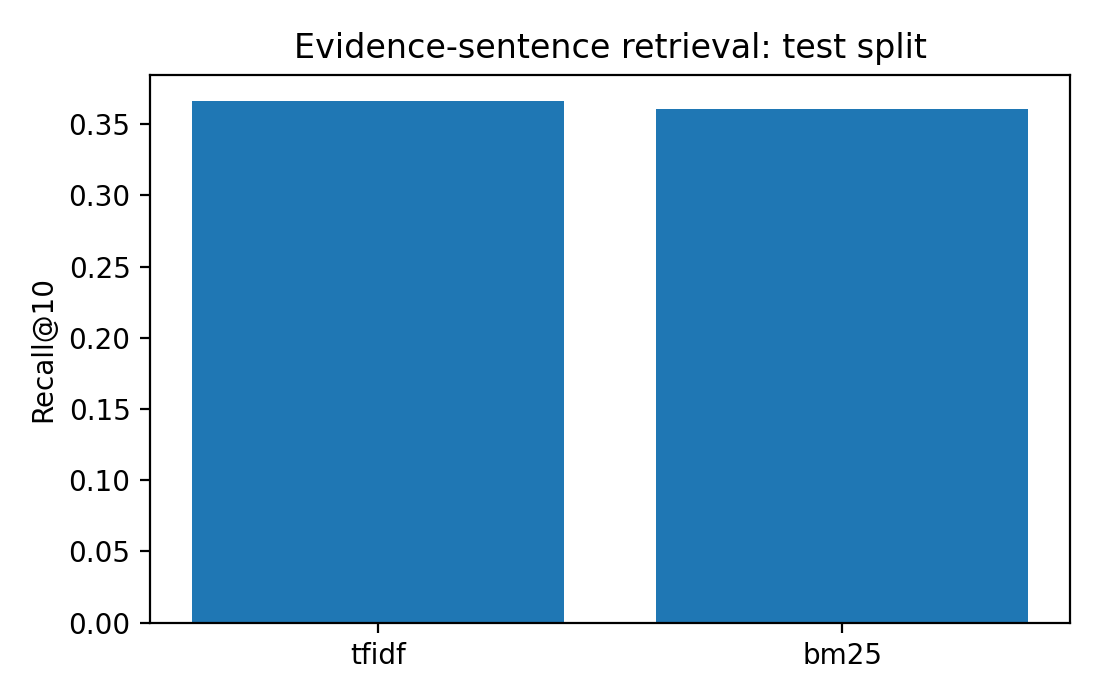
\includegraphics[width=.72\linewidth]{../results/fig_recall_at_10.png}
\caption{Recall@10 on the held-out test split.}
\end{figure}

\section{Lexical-Overlap Analysis}
Development-derived overlap quartile thresholds are 0.3462, 0.4118, and 0.5000. In the highest-overlap test quartile, Recall@10 is 0.4579 for TF--IDF and 0.4630 for BM25. In the lowest-overlap quartile, the corresponding values are 0.3270 and 0.3016. Both methods therefore show better retrieval in the highest-overlap group than in the lowest-overlap group, although the pattern is not strictly monotonic across all four quartiles. This is consistent with lexical retrieval benefiting when the citation context and evidence sentence share more vocabulary, but the observational analysis cannot establish causation.

\begin{figure}[h]
\centering
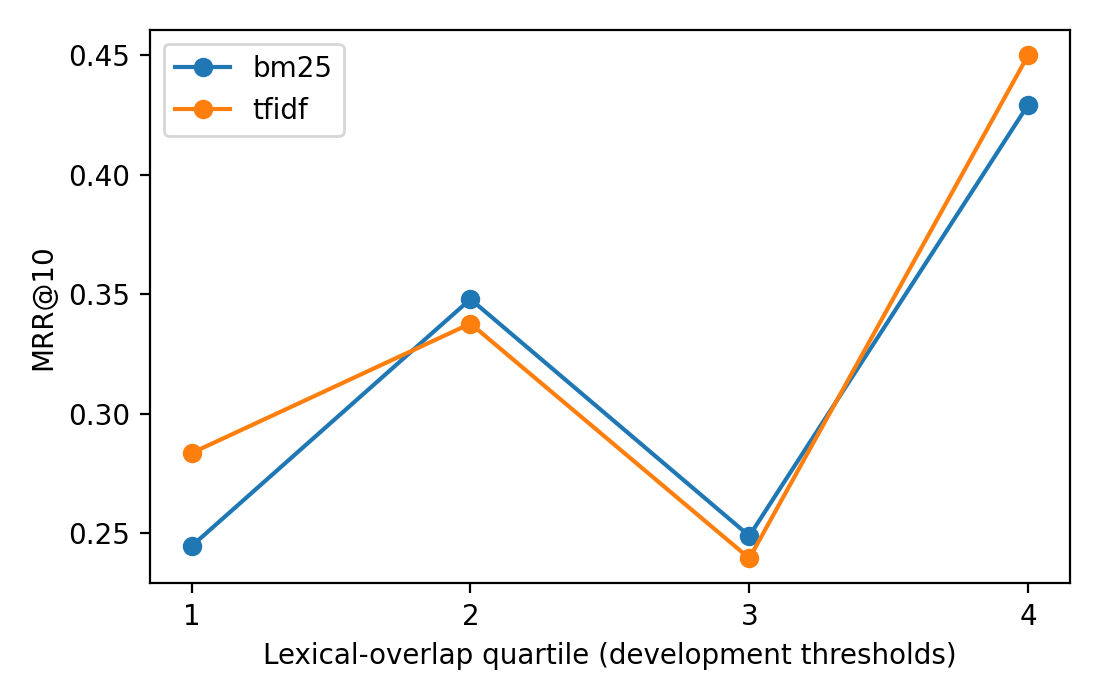
\includegraphics[width=.72\linewidth]{../results/fig_mrr_by_overlap.png}
\caption{MRR@10 across lexical-overlap quartiles, with cutoffs derived from development data.}
\end{figure}

\section{Discussion}
The two lexical baselines are close on the held-out test set. TF--IDF has a small numerical lead in the aggregate metrics, while BM25 slightly exceeds TF--IDF in Recall@10 in the highest-overlap quartile. The paired bootstrap intervals do not support a robust claim that one method is superior. The clearest descriptive pattern is that both methods retrieve evidence more effectively in the highest lexical-overlap group than in the lowest group.

These findings support a restrained conclusion: lexical baselines provide a useful and transparent starting point, but neither is sufficient as a stand-alone solution to citation integrity. A next experiment could compare a dense semantic retriever or a reranker against these lexical baselines under the same article-level split and candidate protocol. Such a comparison should be treated as future work, not as a result of this study.

\section{Limitations}
The candidate set is restricted to sentences in documents enumerated by the dataset's \texttt{cited\_doc\_ids}; it is not an open-web or full-literature retrieval task. The gold annotations may not exhaust every sentence that could support or contextualize a citation. Claims without annotated evidence sentences were excluded from retrieval metrics rather than interpreted as retrieval failures. The methods are lexical and do not include semantic encoders, rerankers, or citation-accuracy classification. The dataset is biomedical and may not generalize to other disciplines. The lexical-overlap analysis is descriptive.

\section{Conclusion}
On the Citation-Integrity test split, TF--IDF and BM25 achieve similar sentence-retrieval performance. TF--IDF is slightly higher in aggregate, but paired bootstrap intervals include zero for Recall@5, Recall@10, and MRR@10. The strongest descriptive pattern is improved retrieval in the highest lexical-overlap quartile. The results do not establish a general winner and do not constitute a complete citation-verification system.

\begin{thebibliography}{9}
\bibitem{sarol2024}
M. J. Sarol, S. Ming, S. Radhakrishna, J. Schneider, and H. Kilicoglu.
\newblock Assessing citation integrity in biomedical publications: corpus annotation and NLP models.
\newblock \emph{Bioinformatics}, 40(7):btae420, 2024.
\newblock doi:10.1093/bioinformatics/btae420.

\bibitem{citationintegrityrepo}
ScienceNLP-Lab.
\newblock Citation-Integrity: Natural language processing to assess and improve citation integrity in biomedical publications.
\newblock \url{https://github.com/ScienceNLP-Lab/Citation-Integrity}.
\end{thebibliography}
\end{document}